\chapter{Initializing Transformers with Residual Flux}
\label{chap:chapter3}
\index{transformer!residual flux}
\index{remanent flux}
\index{inrush current}

\section{General}
\label{sec:section31}
This chapter demonstrates how a transformer model can be initialized with
residual magnetic flux. The examples show how the switching instant and the
polarity of the residual flux determine the maximum core flux and the resulting
magnetizing inrush current.

For an ideal winding, neglecting the winding resistance, the applied voltage
and core flux are related by

\begin{equation}
u(t)=N\frac{\diff\Phi(t)}{\diff t},
\qquad
\Phi(t)=\Phi(0)+\frac{1}{N}\int_0^t u(\tau)\diff\tau.
\label{eq:flux-voltage-integral}
\end{equation}

Consequently, the flux is determined by the time integral of the imposed
voltage and by the initial flux $\Phi(0)$. If a transformer is energized at an
unfavourable point on the voltage waveform, the transient flux can reach twice
its normal steady-state peak. With full residual flux of the same polarity, it
can approach three times the normal peak. Because the core characteristic is
nonlinear, this overfluxing can produce a magnetizing current many times larger
than the normal no-load current.

\begin{important}{Switching instant and residual flux}{Important31}
The initial flux, the voltage phase angle at switching, and the parameter that
applies the initial condition must always be coordinated. A physically
reasonable residual-flux vector in a three-leg core also satisfies approximately
$\Phi_{r0}+\Phi_{s0}+\Phi_{t0}=0$.
\end{important}

\section{Circuit Design}
\label{sec:section32}
For all cases the ltspice file \texttt{Initializing\_Transformers\_with\_residual\_flux.asc} is loaded. 
Four transformer circuits are arranged on the right side of the schematic.
They are supplied at \SI{115}{\kilo\volt}; each transformer is rated
\SI{110}{\kilo\volt}/\SI{10.6}{\kilo\volt}. A switch is placed between each
source and transformer.

The first three circuits are energized at a phase-1 voltage zero crossing and
use different residual-flux settings:

\begin{itemize}
\item no residual flux: \texttt{psi0=0},
\item unfavourable residual flux: \texttt{psi0=1},
\item favourable residual flux: \texttt{psi0=-1}.
\end{itemize}

The fourth circuit is energized at a different point on the voltage waveform
and uses explicitly specified phase residual fluxes. See section 
~\ref{sec:section36}
\begin{remark}{Coordination of initialization time}{remark31}
The transformer parameter \texttt{tpsi0} must match the switch closing time
\texttt{t\_start}. For the first three circuits, use
\begin{lstlisting}[style=LTspice]
t_start=40m  tpsi0=40m
\end{lstlisting}
For the final circuit, use
\begin{lstlisting}[style=LTspice]
t_start=45m  tpsi0=45m
\end{lstlisting}
The \texttt{tpsi0} event rapidly initializes the voltage integrator capacitor
that represents the residual flux.
\end{remark}

\section{Energization at \SI{40}{\milli\second} Without Residual Flux}
\label{sec:section33}
For Trafo1 we set the transformer parameter \texttt{psi0} to zero. The parameter
\texttt{tpsi0} may either be set to \SI{40}{\milli\second} or placed well
outside the simulation interval, for example at \SI{1000}{\second}, because no initial flux has to be applied to Transformer1.

At \SI{40}{\milli\second}, the trace v(phaseA1) voltage starts at zero and initially
becomes positive. Its integral therefore acquires a unidirectional offset. At
\SI{10}{\milli\second} after energization, the phase-1 flux reaches
approximately twice the normal steady-state peak, and the magnetizing current
rises accordingly.

The three phase fluxes can be displayed in the LTspice waveform viewer with

\begin{lstlisting}[style=LTspice]
V(Trafo1:u:_w1:phi)
V(Trafo1:v:_w1:phi)
V(Trafo1:w:_w1:phi)
\end{lstlisting}

Both flux and current decay slowly because a large power transformer has a high
magnetizing inductance and a long electrical time constant. Increasing the
resistance of the source impedance accelerates the decay. This can be examined
with $R=\SI{10}{\ohm}$, \SI{100}{\ohm}, and \SI{1000}{\ohm}.

The rated primary current is approximately \SI{210}{\ampere} RMS. In this
case, the peak magnetizing current is approximately \SI{70}{\ampere}, or about
\SI{50}{\ampere} RMS, and therefore remains below the rated current.

The steady-state peak flux V(trafo1:u:\_w1:phi) is \SI{0.3}{\weber} and the initial flux is 2*\SI{0.3}{\weber}.


\begin{calculation}{Rated steady-state flux}{calculation31} % hier ohne calc: für ref auf gesamte Box 
	% unten mit Calculation~\ref{calc:rated-flux} und 2x compilieren !!!
\begin{align}
\widehat{\Phi}_N
  &=\frac{\sqrt{2}\,U_{\mathrm{ph}}}{\omega N_1}
   =\frac{\sqrt{2}\,U_{\mathrm{LL}}}
          {\sqrt{3}\,\omega N_1}.
          %\label{eq:rated-flux} % für einzelne ref auf formel -> Equation~\eqref{eq:rated-flux}
\end{align}

With $U_{\mathrm{LL}}=\SI{115}{\kilo\volt}$,
$\omega=2\pi\cdot\SI{50}{\hertz}$, and the toolbox default
$N_1=1000$, this gives

\begin{align}
\widehat{\Phi}_N
  &=\frac{\sqrt{2}\cdot\SI{115}{\kilo\volt}}
          {\sqrt{3}\cdot 2\pi\cdot\SI{50}{\hertz}\cdot1000}
    \approx\boxed{\SI{0.299}{\weber}}.
\end{align}
\end{calculation}

\begin{remark}{Line-to-line and phase voltage}{remark32}
For a star-connected three-phase winding, use the phase voltage $U_{ph} = U_{LL}/√3$ and include the RMS-to-peak factor √2 when calculating the peak flux. It is particularly interesting that the magnetic flux depends only on voltage !!! 
\end{remark}

\section{Energization at \SI{40}{\milli\second} with Unfavourable Residual Flux}
\label{sec:section34}

We set \texttt{psi0=1} for Trafo1 . Unless the individual phase parameters are overridden,
the model initializes the phase residual-flux values to

\begin{equation}
(\psi_{r0},\psi_{s0},\psi_{t0})=(1,-0.5,-0.5)\;\text{p.u.}
\end{equation}

Phase 1 therefore starts with full positive residual flux, while phases 2 and
3 start with half the negative value. Since the phase-1 voltage becomes
positive immediately after the switch closes, its integral adds to the
positive residual flux. Approximately \SI{10}{\milli\second} later, the flux
reaches approximately three times the steady-state peak.

The phase-1 current reaches approximately \SI{900}{\ampere} peak. The corresponding RMS value can be calculated in LTspice by zooming in from 40 ms to 60 ms and then left-clicking on the trace name Ix(Trafo2:1U) using the Control button. A pop-up window will then appear, and you can read the RMS value as 380A. This is the procedure to follow if the waveform is not sinusoidal.
The inrush current decays comparatively quickly because the high current
increases the effective damping of the transient.

The corresponding flux traces are

\begin{lstlisting}[style=LTspice]
V(Trafo2:u:_w1:phi)
V(Trafo2:v:_w1:phi)
V(Trafo2:w:_w1:phi)
\end{lstlisting}

The residual-flux values are visible as the initial values at the switching
instant.

\section{Energization at \SI{40}{\milli\second} with Favourable Residual Flux}
\label{sec:section35}

Set \texttt{psi0=-1}. The internal phase residual-flux vector becomes

\begin{equation}
(\psi_{r0},\psi_{s0},\psi_{t0})=(-1,0.5,0.5)\;\text{p.u.}
\end{equation}

The maximum negative phaseA residual flux compensates the positive flux
increment that follows switching at \SI{40}{\milli\second}. Apart from a short
numerical switching spike, the flux moves directly into its steady-state
trajectory and the magnetizing current remains very small.

A similarly smooth startup can be obtained by deleting the switcher and set the Texp parameter of the voltage source to 50ms.

To inspect the small steady-state current in the waveform viewer, manually
limit the current-axis range after the switching spike. The nonlinear
magnetization curve produces a small but visibly distorted current. The phase
fluxes are displayed with ..

\begin{lstlisting}[style=LTspice]
V(Trafo3:u:_w1:phi)
V(Trafo3:v:_w1:phi)
V(Trafo3:w:_w1:phi)
\end{lstlisting}

They are nearly symmetrical with respect to the Y-axis and already settled after energization.

\begin{remark}{Default residual-flux vector}{remark33}
The default vectors $(1,-0.5,-0.5)$ and $(-1,0.5,0.5)$ produce the behaviour
described above only at equivalent points of the \SI{50}{\hertz} waveform,
such as 0, 20, and \SI{40}{\milli\second}. At other switching instants, specify
the individual values with \texttt{psir}, \texttt{psis}, and \texttt{psit}.
\end{remark}

\section{Energization at \SI{45}{\milli\second} with Unfavourable Residual Flux}
\label{sec:section36}

For switching at \SI{45}{\milli\second}, the unfavourable residual-flux vector
differs from the default vector used at the voltage zero crossing. The required
values are as follows:

\begin{lstlisting}[style=LTspice]
psi0=1
psir=0
psis=0.866
psit=-0.866
t_start=45m
tpsi0=45m
\end{lstlisting}

With these settings, the phaseA current is the smallest, whereas the currents
in phases 2 and 3 are the largest. The currents remain high, but their maxima
are lower than in the unfavourable \SI{40}{\milli\second} case seen in section
\ref{sec:section34}.\\
%\vspace{0.5cm}

The phase fluxes can be displayed with ..
\begin{lstlisting}[style=LTspice]
V(Trafo4:u:_w1:phi)
V(Trafo4:v:_w1:phi)
V(Trafo4:w:_w1:phi)
\end{lstlisting}

\begin{figure}[H]
	\centering
	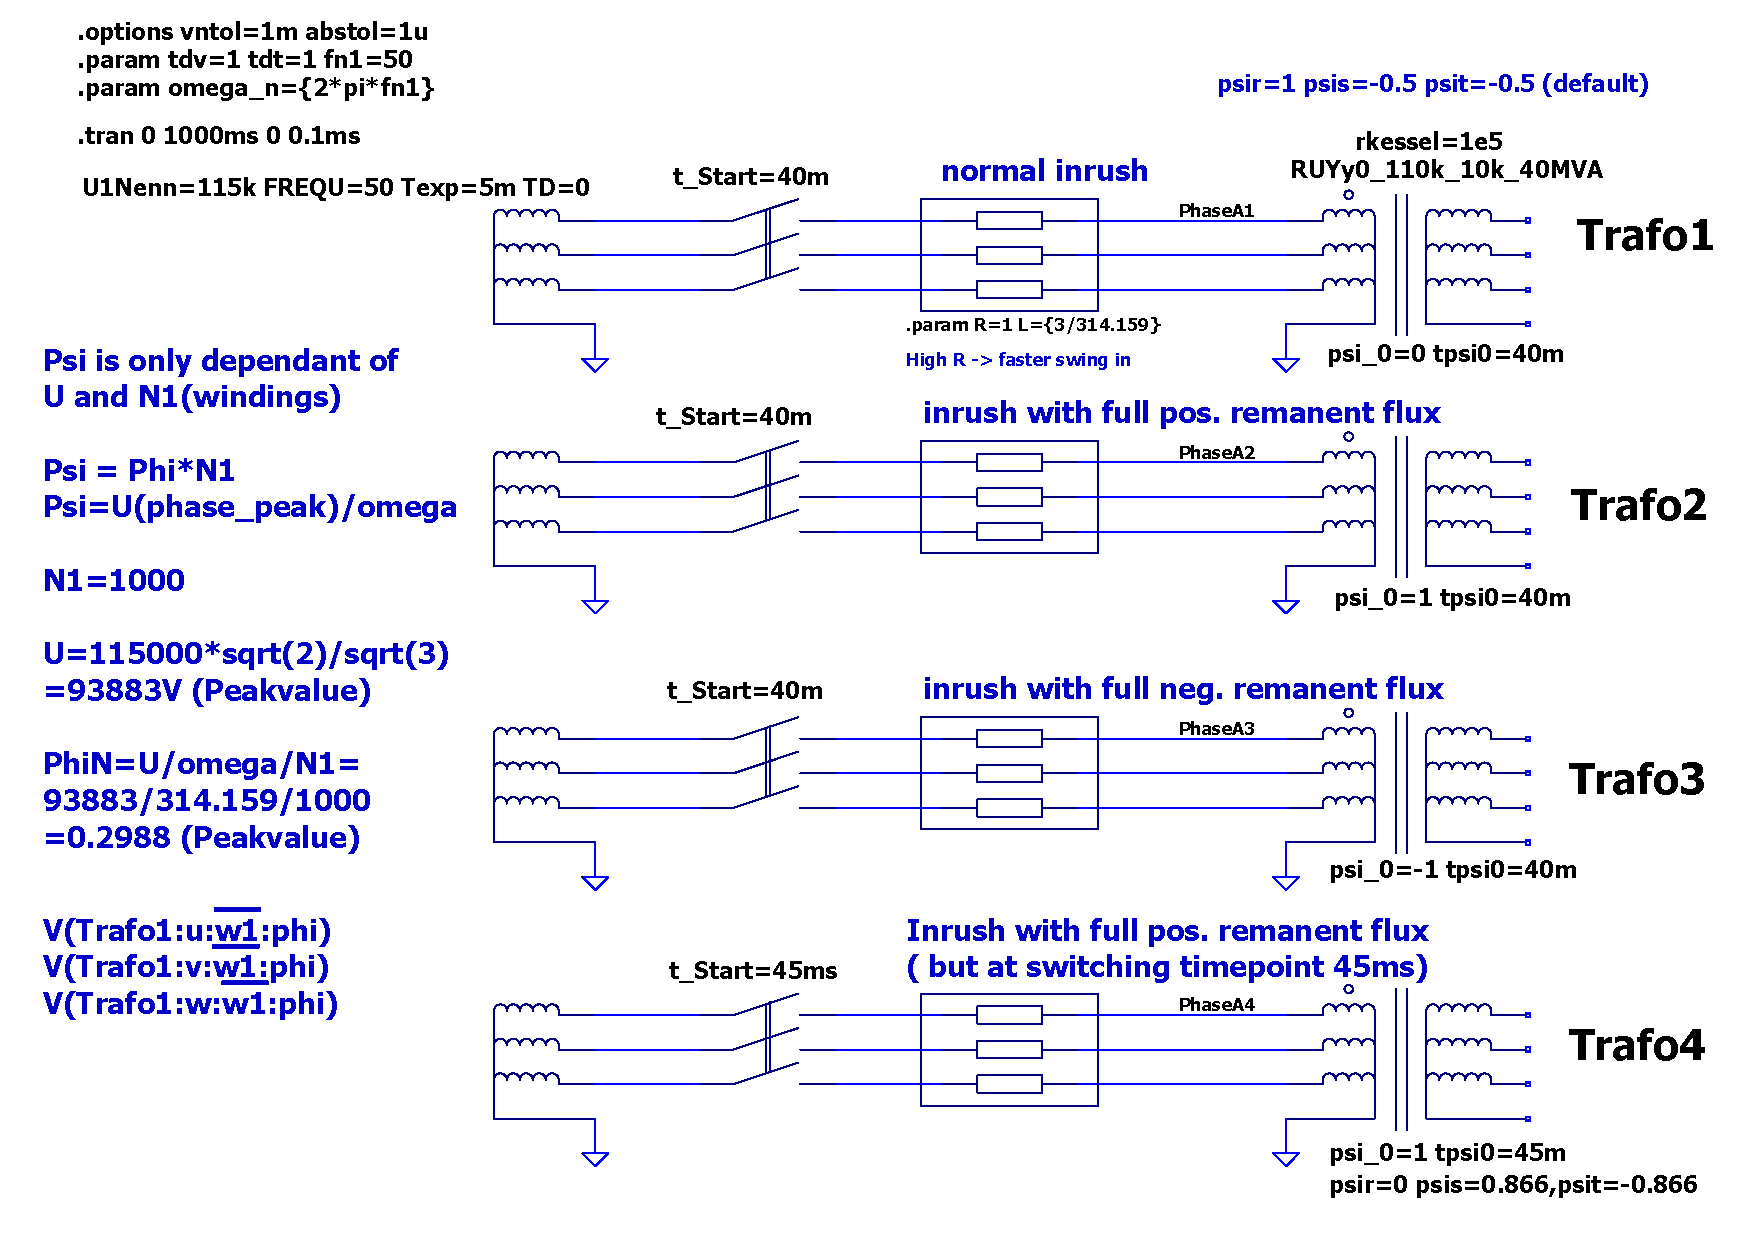
\includegraphics[width=1\textwidth] {figures/03_Initializing_Transformers_with_residual_flux/Initializing_Transformers_with_remanent_flux_Schematic}
	\caption{Initializing a Transformer with residual flux - schematic}
	\label{fig:figure31}
\end{figure}

\begin{figure}[H]
	\centering
	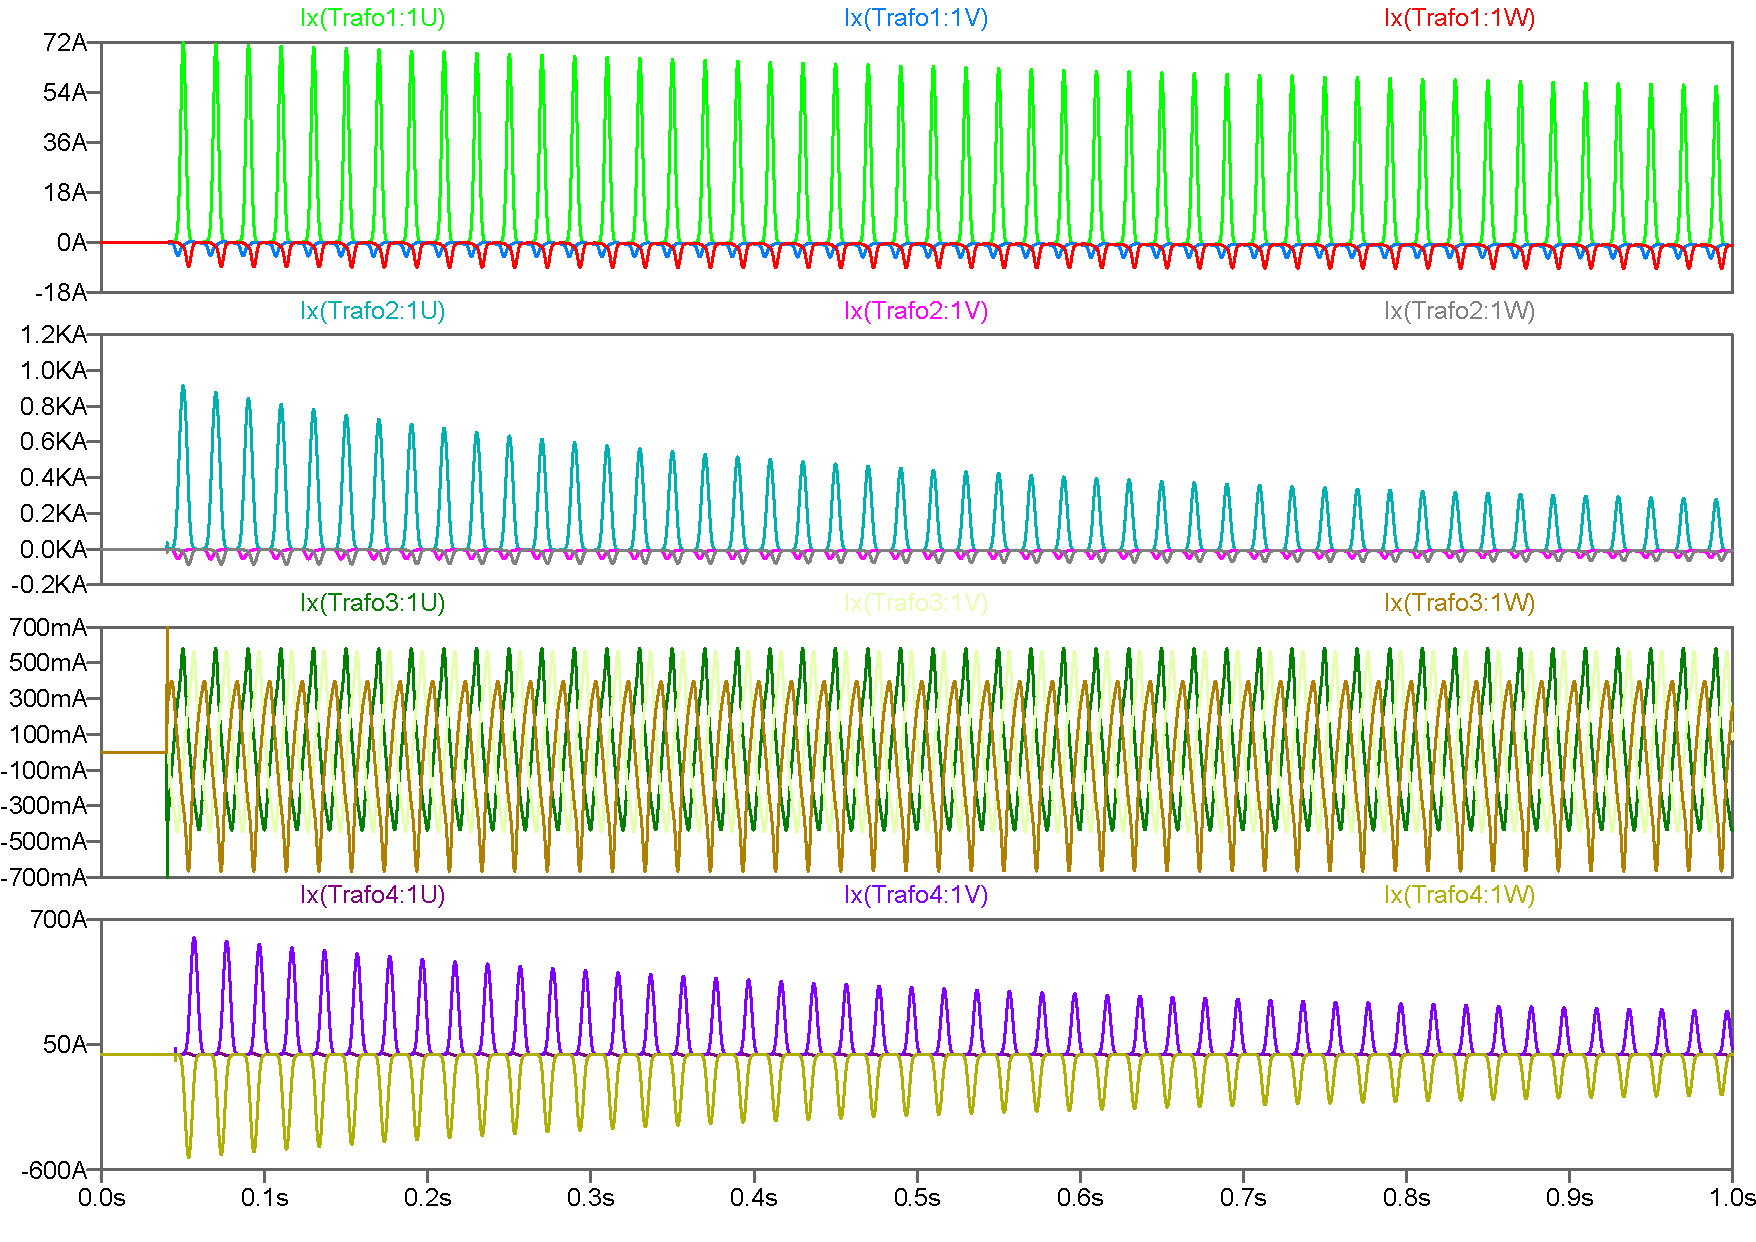
\includegraphics[width=0.9\textwidth] {figures/03_Initializing_Transformers_with_residual_flux/Initializing_Transformers_with_remanent_flux_waveform_of_currents}
	\caption{Initializing a Transformer with residual flux - Currents}
	\label{fig:figure32}
\end{figure}

\begin{figure}[H]
	\centering
	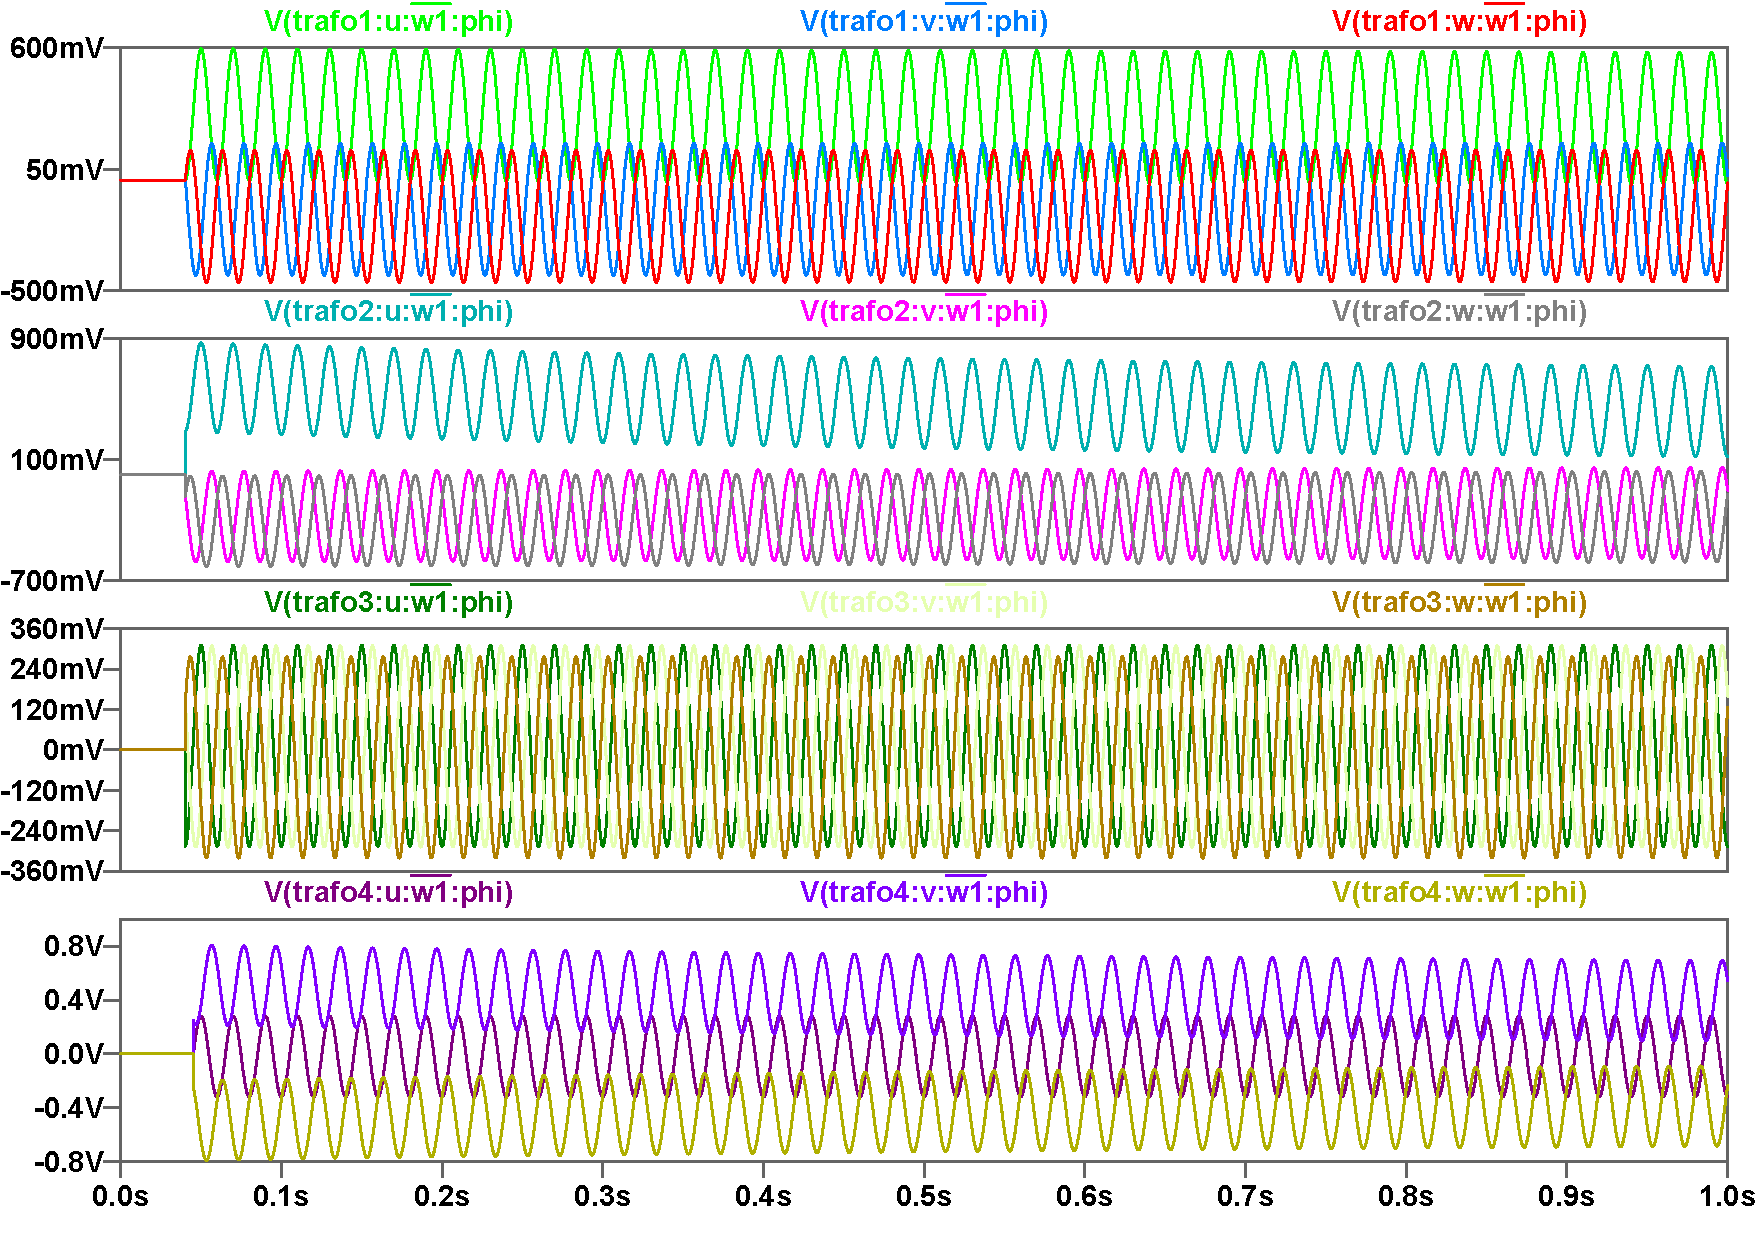
\includegraphics[width=0.9\textwidth] {figures/03_Initializing_Transformers_with_residual_flux/Initializing_Transformers_with_remanent_flux_waveform_of_fluxes}
	\caption{Initializing Transformer with residual flux - Fluxes}
	\label{fig:figure33}
\end{figure}


\begin{chaptersummary}
Transformer energization is governed by the integral of the applied voltage
and by the residual core flux at the switching instant. Closing at a voltage
zero crossing without residual flux can produce approximately twice the normal
steady-state peak flux. Unfavourable full residual flux can increase this to
about three times the normal peak and cause a large inrush current. Favourable
residual flux, controlled switching, or a gradual source-voltage ramp can
greatly reduce the transient. The initialization time and all three phase
residual-flux values must be coordinated with the switch closing instant.
Hint: It is often mentioned in the literature that the inrush current is attenuated by connecting the transformer to a load. However, this is not the case unless the load is truly very high—which, in turn, causes the total current to be very high, thereby masking the inrush current.
See LTspice example \texttt{Hidden\_inrush.asc} in this example folder
\end{chaptersummary}
